\documentclass[a4paper,oneside,12pt]{book}

%----------------------------------------------------------------------------------------
%	README!
%   Welcome. It's worth having a read through this file
%   to set up the broad parameters, such as the name of
%   the degree, the school/department, the type of work
%   (dissertation/Final Year Project/report, etc. as well
%   as your own details.
%----------------------------------------------------------------------------------------

%----------------------------------------------------------------------------------------
%	COVER PAGE
%   The cover page is laid out in title/title.tex. You can choose a colour
%   or black and white logo
%----------------------------------------------------------------------------------------

%----------------------------------------------------------------------------------------
%	THESIS INFORMATION
%   Put title, author name, degree, type of work, school, department in here
%   It will be used for the title page and for the embedded PDF information
%----------------------------------------------------------------------------------------

\newcommand{\thesistitle}{Title of Work} % Your thesis title, this is used in the title and abstract
\newcommand{\degree}{MAI (Computer Engineering)} % Your degree name, this is used in the title page and abstract
\newcommand{\typeofthesis}{dissertation} % dissertation, Final Year Project, report, etc.
\newcommand{\authorname}{Dara \'O S\'uilleabh\'ain} % Your name, this is used in the title page and PDF stuff
%% Do not put your Student ID in the document, as TCD will not publish
%% documents that contain both your name and your Student ID.

\newcommand{\keywords}{this, that, more} % Keywords for your thesis
\newcommand{\school}{\href{http://www.scss.tcd.ie}{School of Computer Science and Statistics}} % Your school's name and URL, this is used in the title page

%% Comment out the next line if you don't want a department to appear
%\newcommand{\department}{\href{http://researchgroup.university.com}{Department Name}} % Your research group's name and URL, this is used in the title page

\AtBeginDocument{
\hypersetup{pdftitle=\thesistitle} % Set the PDF's title to your title
\hypersetup{pdfauthor=\authorname} % Set the PDF's author to your name
\hypersetup{pdfkeywords=\keywords} % Set the PDF's keywords to your keywords
\hypersetup{pdfsubject=\degree} % Set the PDF's keywords to your keywords
}

%% Language and font encodings
\usepackage[T1]{fontenc} 
\usepackage[utf8]{inputenc}
\usepackage[english]{babel}

%% Bibliographical stuff
\usepackage[round,sort,comma,numbers]{natbib}

%% Document size
% include showframe as an option if you want to see the boxes
\usepackage[a4paper,top=2.54cm,bottom=2.54cm,left=2.54cm,right=2.54cm,headheight=16pt]{geometry}
\setlength{\marginparwidth}{2cm}
%% Useful packages
\usepackage{amsmath}
\usepackage[autostyle=true]{csquotes} % Required to generate language-dependent quotes in the bibliography
\usepackage[pdftex]{graphicx}
\usepackage[colorinlistoftodos]{todonotes}
\usepackage[colorlinks=true, allcolors=black]{hyperref}
\usepackage{caption} % if no caption, no colon
\usepackage{sfmath} %use sans-serif in the maths sections too
\usepackage[parfill]{parskip}    % Begin paragraphs with an empty line rather than an indent
\usepackage{setspace} % to permit one-and-a-half or double spacing
\usepackage{enumerate} % fancy enumerations like (i) (ii) or (a) (b) and suchlike
\usepackage{booktabs} % To thicken table lines
\usepackage{fancyhdr}

\pagestyle{plain} % Embrace simplicity!

%% The Mechanical engineers require your name and ID on the top of every page.
%% Uncomment the following block if you want your name and ID at the top of
%% (almost) every page.

%\pagestyle{fancy}
%\fancyhf{} % sets both header and footer to nothing
%\renewcommand{\headrulewidth}{0pt}
%\cfoot{\thepage}
%\ifdefined\authorid
%\chead{\it \authorname\ (\authorid)}
%\else
%\chead{\it \authorname}
%\fi
%% End of block

%% It is not a requirement of the university that the font should be sans-serif, but
%% the Mechanical engineers require it. Comment out the following line to disable it
\renewcommand{\familydefault}{\sfdefault} %use the sans-serif font as default

%% If you're not using sans-serif, consider using Palatino instead of the LaTeX standard
%\usepackage{mathpazo} % Use the Palatino font by default if you prefer it to Computer Modern

\renewcommand{\theequation}{\arabic{equation}} %% use continuous equation numbers

%% Format Chapter headings appropriately
\usepackage{titlesec}
\titleformat{\chapter}[hang] 
{\normalfont\huge\bfseries}{\thechapter}{1cm}{} 

\title{\thesistitle}
\author{\authorname}

\frontmatter
\begin{document}
\begin{titlepage}

\center % Center everything on the page

%% All the text parameters should be taken from the start of the main.tex file.
%% You should only alter stuff here if you want to change the layout

%----------------------------------------------------------------------------------------
%	LOGO SECTION
%----------------------------------------------------------------------------------------
%% Choose one of the following -- a colour or black-and-white logo


\includegraphics{title/Trinity_RGB_transparent_main.png}\\[1cm] 
%
\includegraphics[width=12cm]{title/black-stacked-trinity.jpg}\\[1cm] 

\Large \school\\[1.5cm] % Minor heading such as course title
\ifdefined\department
\large \department\\[1.5cm] % Minor heading such as course title
\fi

%----------------------------------------------------------------------------------------
%	TITLE SECTION
%----------------------------------------------------------------------------------------
\makeatletter
{ \huge \bfseries \thesistitle}\\[1.5cm] % Title of your document
 

%----------------------------------------------------------------------------------------
%	AUTHOR SECTION
%----------------------------------------------------------------------------------------

\ifdefined\authorid
\authorname\\ % Your name
\authorid\\[2cm] % Your Student ID
\else
\authorname\\[2cm] % Your name
\fi

%----------------------------------------------------------------------------------------
%	DATE SECTION
%----------------------------------------------------------------------------------------

{\large \today}\\[2cm] % Date, change the \today to a set date if you want to be precise

 
%----------------------------------------------------------------------------------------
%	TYPE OF THESIS SECTION
%----------------------------------------------------------------------------------------
\vfill
 A \typeofthesis\ submitted in partial fulfilment\\of the requirements for the degree of\\
\degree

\vfill % Fill the rest of the page with whitespace

\end{titlepage}
\pagenumbering{roman}
\section*{\Huge{Declaration}}
\vspace{1cm}
I hereby declare that this \typeofthesis\ is entirely my own work and that it has not been submitted as an exercise for a degree at this or any other university.

\vspace{1cm}
I have read and I understand the plagiarism provisions in the General Regulations of the University Calendar for the current year, found at \url{http://www.tcd.ie/calendar}.
\vspace{1cm}

I have also completed the Online Tutorial on avoiding plagiarism `Ready Steady Write', located at \url{http://tcd-ie.libguides.com/plagiarism/ready-steady-write}.
\vspace{3cm}

Signed:~\rule{5cm}{0.3pt}\hfill Date:~\rule{5cm}{0.3pt}

\chapter*{Abstract}
A short summary of the problem investigated, the approach taken and the key findings. This should not be more that around 400 words.

The must be on a separate page.

\newpage
\onehalfspacing\raggedright %\raggedright turns off justification and hypenation

\section*{\Huge{Acknowledgements}}
Thanks Mum!

You should acknowledge any help that you have received (for example from technical staff), or input provided by, for example, a company.
\tableofcontents
\listoffigures
\listoftables
\newpage
\section*{\Huge{Nomenclature}}
\begin{tabular}{lp{9cm}l}
A&Area of the wing&$m^{2}$\\
B\\
C& Roman letters first, with capitals\ldots\\
a&then lower case.\\
b\\
c\\
$\Gamma$&Followed by Greek capitals\ldots\\
$\alpha$&then lower case greek symbols.\\
$\beta$\\
$\epsilon$\\
TLA&Finally, three letter acronyms and other abbreviations arranged alphabetically\\
\end{tabular}
\vspace{2cm}

If a parameter has a typical unit that is used throughout your report, then it should be included here on the right hand side.

If you have a very mathematical report, then you may wish to divide the nomenclature list into functions and variables, and then sub- and super-scripts.

Note that Roman mathematical symbols are typically in a serif font in italics.

\mainmatter
\chapter{Introduction}
\label{chap:Introduction}
This chapter introduces the background \ref{sec:Research background} of the current COVID-19 pandemic, leading to the research questions and aims \ref{sec:Research aims} to be achieved in this research.
Furthermore, since human participants are involved in data collection and model training, research ethics \ref{sec:Research ethics} are discussed. Finally, this chapter also presents the overview and structure \ref{sec:Dissertation overview} of this dissertation.
\section{Research background}
\label{sec:Research background}
%2 pages
%COVID-19 impacts education
COVID-19 has brought many challenges to higher education.
\citet{marinoni2020impact} reiterate the facts released by UNESCO regarding the significant impact of the pandemic on education in countries around the world.
For example, there are approximately 130 million students, accounting for 89.4\% of total enrolled learners, whose academic career has been vitiated because of the impact of pervading virus caused school closures.

To better respond to the crisis and allay public concerns caused by the epidemic, the International Association of Universities (IAU) launches a survey of the impact of COVID-19 on higher education.
\citet{marinoni2020impact} present the survey results showing that COVID-19 has inevitably affected many processes in education, including teaching \& learning, researching, and assessment.

In teaching and learning, most classroom lectures have been substituted by distance teaching and learning, which may not be difficult for professors and students who are familiar with computers and the Internet.
On the other hand, experiments and research that require the use of shared professional equipment are much more severely affected.
The survey shows that 80\% of researchers have reported that their research progress is decelerating and moving at a creep.

However, as for assessment and examination, institutions have no way to perpetuating the traditional assessment methods, which is indicated by \citet{clark2020testing} as one of the most important challenges for students.
``Learning assessment and examination approaches will be reviewed, and institutions may choose to invest further in technical infrastructures'', said by \citet{marinoni2020impact} points out the fact.
Although some universities shift from closed-book exams to pure continuous assessments immediately, other educational institutions are craving for new technologies to help them out of trouble.

As a result, the motivation of this research is to investigate the feasibility of deep-learning-based human action recognition techniques in the distance invigilation application and provide a way for educational institutions to hold exams and reduce labour costs.

%Deep learning technologies are widely used, applications
In recent years, ubiquitous influences of deep learning methods have brought tremendous advancement to many computer science fields and individual's daily life. 
In many fields, such as computer vision and natural language processing, deep learning approaches achieved higher performance than traditional algorithms.
\citet{mccay2020abnormal} show that in the research field of automatic human action recognition, the analysis and reconstruction of human actions have copious applications, including content-based video indexing, intelligent surveillance, human-computer interaction, and virtual reality.
Therefore, this research will explore deep learning techniques to solve automatic exam invigilation problems in the assessment process of distance education.

This research is also based on previous studies in deep learning and deep model mobilisation.
Currently, there are some existing models for human posture analysis and detection.
But many of them use static imagery as input and key points of the body as output, and they are not optimised for mobile devices with limited computing power.
Beside, the personal computer hardware, the bridge between the software system and the physical space, is not trusted.
However, a trusted software environment can be ensured on mobile phones with hardware attestation functions provided by operating system and device manufactures.


\section{Research aims}
\label{sec:Research aims}
%1 page
After clarifying the research background, the research question of this dissertation is summarised as the following:

\begin{quote}
    Is it possible to understand sequential human actions from an on-device camera video input stream with deep learning technologies to classify the series of actions of the exam attendee to approved or prohibited behaviours with high accuracy?
\end{quote}

In order to answer the research question, this research aims to achieve the objectives through the corresponding methods shown in Table \ref{tab:Research objectives}.

\begin{table}[!ht]
    \centering
    \begin{longtable}{>{\hspace*{-0.3cm}$\bullet$\hspace*{0.2cm}}p{.4\textwidth}p{.56\textwidth}}
\textbf{Research objectives} & \textbf{Method to achieve objectives} \\ \hline
To do the literature review & By surveying the state-of-the-art technologies of deep-learning-based human action recognition \\ \hline
To have an available data set & By obtaining a suitable image and video data set and labelling them for training the model \\ \hline
To design a deep learning model & By designing a deep learning model \\ \hline
To code and train the deep model & By training the model and fine-tuning hyper-parameters \\ \hline
To optimise the model for mobile & By developing a working mobile app that equips the model \\ 
\end{longtable}
    \caption{Research objectives and corresponding methods}
    \label{tab:Research objectives}
\end{table}

After completing the above objectives, this research will also evaluate the project outcomes, especially for model performance and other following aspects.

\begin{itemize}
    \item Model accuracy, precision and other evaluation metrics on the classification task.
    \item Balanced performance between accuracy and efficiency of the deep learning model.
    \item User experiences of the overall system.
\end{itemize}


\section{Research ethics}
\label{sec:Research ethics}
%2 pages

\section{Dissertation overview}
\label{sec:Dissertation overview}
%.5 page
This dissertation comprises six chapters, beginning with this introduction chapter \ref{chap:Introduction}, presenting the research background, aims and ethics, followed by the literature review chapter \ref{chap:Literature review}, which comprehensively reviews previous researches on deep learning models and the related state-of-the-art works.
In chapter \ref{chap:Design}, this dissertation proposes the deep learning model used to recognise and classify actions, based on various designing trade-offs and mobile optimisation methods learned from previous research.
Figure \ref{fig:0-Intro-Overview} shows the project overview, in which these process pipelines and the proposed deep learning model are implemented in chapter \ref{chap:Implementation}.
Further, the experiments are conducted

\begin{figure}[h]
    \centering
    \hspace*{-.5cm}
    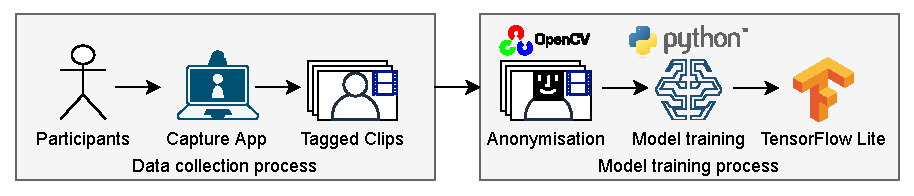
\includegraphics[scale=1.1]{introduction/imgs/0-Intro-Overview.pdf}
    \caption{Project overview}
    \label{fig:0-Intro-Overview}
\end{figure}

\chapter{Background}

\chapter{\LaTeX}
\label{latexchapter}
\LaTeX{}, or more properly ``\LaTeXe{}'', is a very useful document processing program. It is very widely used, widely available, stable and free. Famously, \TeX, upon which \LaTeX{} is built, was originally developed by the eminent American mathematician Donald Knuth because he was tired of ugly mathematics books \cite{shustek2008interview}. Although it has a learning curve (made much less forbidding by online tools and resources -- see below), it allows the writer to concentrate more fully on the content, and takes care of most everything else.

While it can be used as a word processor, it is a \emph{typesetting} system, and Knuth's idea was that it could be used to produce beautiful looking books:
\begin{quote}
\emph{\LaTeX{} is a macro package which enables authors to typeset and print their work at the highest typographical quality, using a predefined, professional layout.}\footnote{This is from \citet{oetiker2001not}. Did we mention that you should minimise your use of footnotes?}
\end{quote}
\LaTeX{} has great facilities for setting out equations and a powerful and very widely supported bibliographic system called BibTeX, which takes the pain out of referencing.

Three useful online resources make \LaTeX~much better:
\begin{enumerate}[(1)]
\item An excellent online \LaTeX{} environment called ``Overleaf'' is available at \url{http://www.overleaf.com} and runs in a modern web browser. It's got this template available -- search for a TCD template. Overleaf can work in conjunction with Dropbox, Google Drive and, in beta, GitHub.
\item Google Scholar, at \url{http://scholar.google.com}, provides BibTeX entries for most of the academic references it finds.
\item An indispensable and very fine introduction to using \LaTeX{} called \emph{``The not so short introduction to LATEX 2$\varepsilon$''} by \citet{oetiker2001not} is online at \url{https://doi.org/10.3929/ethz-a-004398225}. Browse it before you use \LaTeX~for the first time and  read it carefully when you get down to business.
\end{enumerate}
Other tools worth mentioning include:
\begin{itemize}
\item \texttt{Draw.io} -- an online drawing package that can output PDFs to Google Drive -- see \url{https://www.draw.io}.
\end{itemize}
\chapter{Evaluation}
\label{chap:Evaluation}
% 10 pages
\section{Evaluation metrics}
\label{sec:Evaluation metrics} % 2 pages
\section{Model training}
\label{sec:Model training} % 2 pages
\section{Visual results}
\label{sec:Visual results} % 4 pages
\section{Comparison with other solutions}
\label{sec:Comparison with other solutions} % 2 pages

\chapter{Conclusion}
\label{chap:Conclusion}
% 1 page discussion and summary, 1 page possible future works
In the previous section, each part of the system was evaluated with some key result data listed in tables.
This section will discuss on the results to draw research conclusions and propose some possible future works in this field.

% Future works
A deep learning library for video understanding research\footnote{PyTorchVideo: \url{https://github.com/facebookresearch/pytorchvideo}}

\bibliographystyle{unsrtnat}
\bibliography{bibs/sample}
\appendix
\renewcommand{\thechapter}{A\arabic{chapter}}
\chapter{Appendix}
You may use appendices to include relevant background information, such as calibration certificates, derivations of key equations or presentation of a particular data reduction method. You should not use the appendices to dump large amounts of additional results or data which are not properly discussed. If these results are really relevant, then they should appear in the main body of the report.

\section{Appendix numbering}
Appendices are numbered sequentially, A1, A2, A3\ldots The sections, figures and tables within appendices are numbered in the same way as in the main text. For example, the first figure in Appendix A1 would be Figure A1.1. Equations continue the numbering from the main text.



\end{document}